\documentclass[10pt, twocolumn]{article}

% ======================================================================
% PACKAGES & SETUP
% ======================================================================
\usepackage[utf8]{inputenc}
\usepackage{graphicx}      % For including figures
\usepackage{booktabs}      % For professional tables
\usepackage{hyperref}      % For hyperlinks
\usepackage{geometry}      % For page margins
\usepackage{authblk}       % For author affiliation
\usepackage{amsmath}       % For math formatting
\usepackage{float}         % For figure placement
\usepackage{caption}       % For caption formatting
\usepackage{subcaption}    % For subfigures
\usepackage{listings}      % For code snippets in appendices
\usepackage{xcolor}        % For code coloring

% Geometry Setup
\geometry{a4paper, margin=2cm}

% Code Listing Style
\lstset{
    basicstyle=\ttfamily\small,
    breaklines=true,
    frame=single,
    backgroundcolor=\color{gray!10},
    captionpos=b
}

% Title Data
\title{\textbf{Neuromodulated Language Models: Prototyping Pharmacological Analogues and Blind, Placebo-Controlled Evaluation}}
\author[1]{The Neuromodulation Research Group}
\affil[1]{Department of Computational Psychopharmacology}
\date{\today}

\begin{document}

\maketitle

% ======================================================================
% ABSTRACT
% ======================================================================
\begin{abstract}
We introduce and evaluate a suite of inference-time ``neuromodulation packs'' that mimic canonical neurochemical effects (e.g., serotonergic psychedelics, stimulants, depressants) in large language models. Using a double-blind, placebo-controlled, within-model crossover design ($N=13$ packs, $n=126$ trials per condition), we benchmark behavioral signatures against human subjective-effect profiles. Our results demonstrate a functional isomorphism between biological gain control and computational inference steering: the \textbf{Serotonergic Agonist} class (LSD, Psilocybin) reliably induced high-entropy altered states ($p < 0.001$, $d=10.0$) detectable via the novel \textit{Psychedelic Detection Questionnaire} (PDQ-S). Conversely, \textbf{Stimulant} packs failed to surpass the baseline focus of the reinforcement-learned model, suggesting a ``focus ceiling'' effect. We discuss implications for dynamic, reversible AI alignment via digital psychopharmacology.
\end{abstract}

\textbf{Keywords:} neuromodulation; inference-time control; activation steering; KV-cache; psychedelics; stimulants; placebo-controlled; blind evaluation; LLM

% ======================================================================
% 1. INTRODUCTION
% ======================================================================
\section{Introduction}
In biological neural networks, the transition between distinct behavioral states—from the hyper-associative fluidity of a dream to the rigid, goal-directed focus of a hunt—is not mediated by rewiring connections, but by \textit{neuromodulation}. A wash of serotonin or a burst of norepinephrine acts as a global gain control mechanism, shifting the operating regime of cortical circuits without altering their underlying topology. We propose that this biological architecture offers more than just a metaphor for Artificial Intelligence; it provides a functional blueprint for the inference-time control of Large Language Models (LLMs).

Current paradigms for controlling LLM behavior typically rely on fine-tuning (analogous to synaptic learning) or prompting (analogous to sensory input). However, a third path exists: direct manipulation of the computational substrate during inference. Recent advances in activation steering \cite{turner2023, rimsky2023}, KV-cache surgery \cite{xiao2023}, and decoding-time intervention \cite{liu2021} allow us to intervene in the model's ``cognitive'' process as it unfolds.

We frame these disparate computational interventions as \textbf{``neuromodulation packs''}—discrete, portable configurations of hyperparameters and steering vectors designed to mimic the functional effects of specific neurochemical classes. By treating the residual stream as a carrier of ``cognitive state'' and the attention mechanism as a ``routing gate,'' we can induce reversible, drug-like states in an LLM. For instance, we model the effects of \textbf{Serotonergic Psychedelics} not by prompting the model to ``act trippy,'' but by injecting entropy and orthogonal steering vectors that mathematically destabilize semantic attractors—a computational implementation of the Entropic Brain Hypothesis \cite{carhart2014}.

This paper presents a double-blind, placebo-controlled, within-model crossover study evaluating these packs. By subjecting Llama-3.1-8B to a battery of ``digital psychometric'' tests, we demonstrate that biological gain control mechanisms have a direct computational isomorphism in transformer architectures, offering a new primitive for dynamic, reversible AI alignment.

% ======================================================================
% 2. RELATED WORK
% ======================================================================
\section{Related Work}

\subsection{Activation Steering and Representation Engineering}
The direct manipulation of internal model representations has emerged as a powerful alternative to prompting. Turner et al. (2023) and Rimsky et al. (2023) introduced \textit{activation steering} (or ``activation engineering''), demonstrating that adding a fixed ``steering vector'' to the residual stream during the forward pass can reliably elicit specific behaviors, such as truthfulness or refusal. Rimsky's work on \textit{Contrastive Activation Addition (CAA)} is particularly relevant, as it provides a method for deriving these vectors by averaging the difference in activations between positive and negative prompt pairs. Our work extends this by grouping multiple steering vectors into ``packs'' that target broad behavioral phenotypes rather than single tasks.

\subsection{Decoding-Time Control}
Prior to activation steering, control was often exerted at the sampling stage. The \textit{Plug and Play Language Model (PPLM)} utilized gradients from an external attribute classifier to update hidden states during generation. Later approaches like \textit{GeDi} and \textit{DExperts} employed smaller ``expert'' and ``anti-expert'' language models to guide the logits of a larger base model. While effective, these methods often require auxiliary models. Our ``Stimulant'' packs approximate these effects using lightweight logits processors (e.g., presence penalties, dynamic temperature) to sharpen focus without the overhead of external classifiers.

\subsection{KV-Cache and Attention Manipulation}
Efficient long-context inference has driven research into managing the Key-Value (KV) cache. Xiao et al. (2023) introduced \textit{StreamingLLM}, identifying ``attention sinks''—initial tokens that garner disproportionate attention—and demonstrating that stable inference can be maintained even when evicting the vast majority of the cache. We repurpose this ``eviction'' mechanism for our ``Depressant'' packs: rather than optimizing for efficiency, we strategically induce ``forgetting'' (simulated amnesia) by aggressively decaying the KV-cache, analogous to the GABAergic inhibition of working memory.

\subsection{The Entropic Brain Hypothesis}
Our theoretical framework for the ``Psychedelic'' packs draws directly from the \textit{Entropic Brain Hypothesis} \cite{carhart2014}. This theory posits that the quality of conscious states correlates with the entropy of brain activity, and that psychedelics work by increasing this entropy, collapsing the rigid ``priors'' of the Default Mode Network (DMN). We translate this into the transformer domain by treating the model's ``safety rails'' and canonical semantic pathways as the DMN, and using high-temperature sampling and noise injection to fundamentally destabilize these priors.

% ======================================================================
% 3. METHODS
% ======================================================================
\section{Methods}

\subsection{Models and Serving Stacks}
Our primary experiments were conducted on \textbf{Llama-3.1-8B-Instruct}, a dense transformer model with 8 billion parameters. The experimental framework utilizes Hugging Face Transformers with custom hooks for activations, attention, and KV-cache manipulation. All models run locally, as API-based models (OpenAI, Anthropic) lack access to model internals required for activation effects, attention manipulation, and KV-cache surgery.

\subsection{Neuromodulation Packs (Implementation)}
We define a ``neuromodulation pack'' as a tuple $P = (\Theta_{sample}, \mathcal{T}_{steer}, \Phi_{mem})$ containing parameters for sampling, activation steering, and memory manipulation. These packs are applied at inference time via the \texttt{NeuromodulationTool} API, which intercepts the generation process at three levels: (1) the sampler, (2) the residual stream (steering vectors), and (3) the KV-cache. The \texttt{NeuromodulationTool} wraps the base model and intercepts the forward pass to apply these interventions.

% FIGURE 1
\begin{figure}[ht]
    \centering
    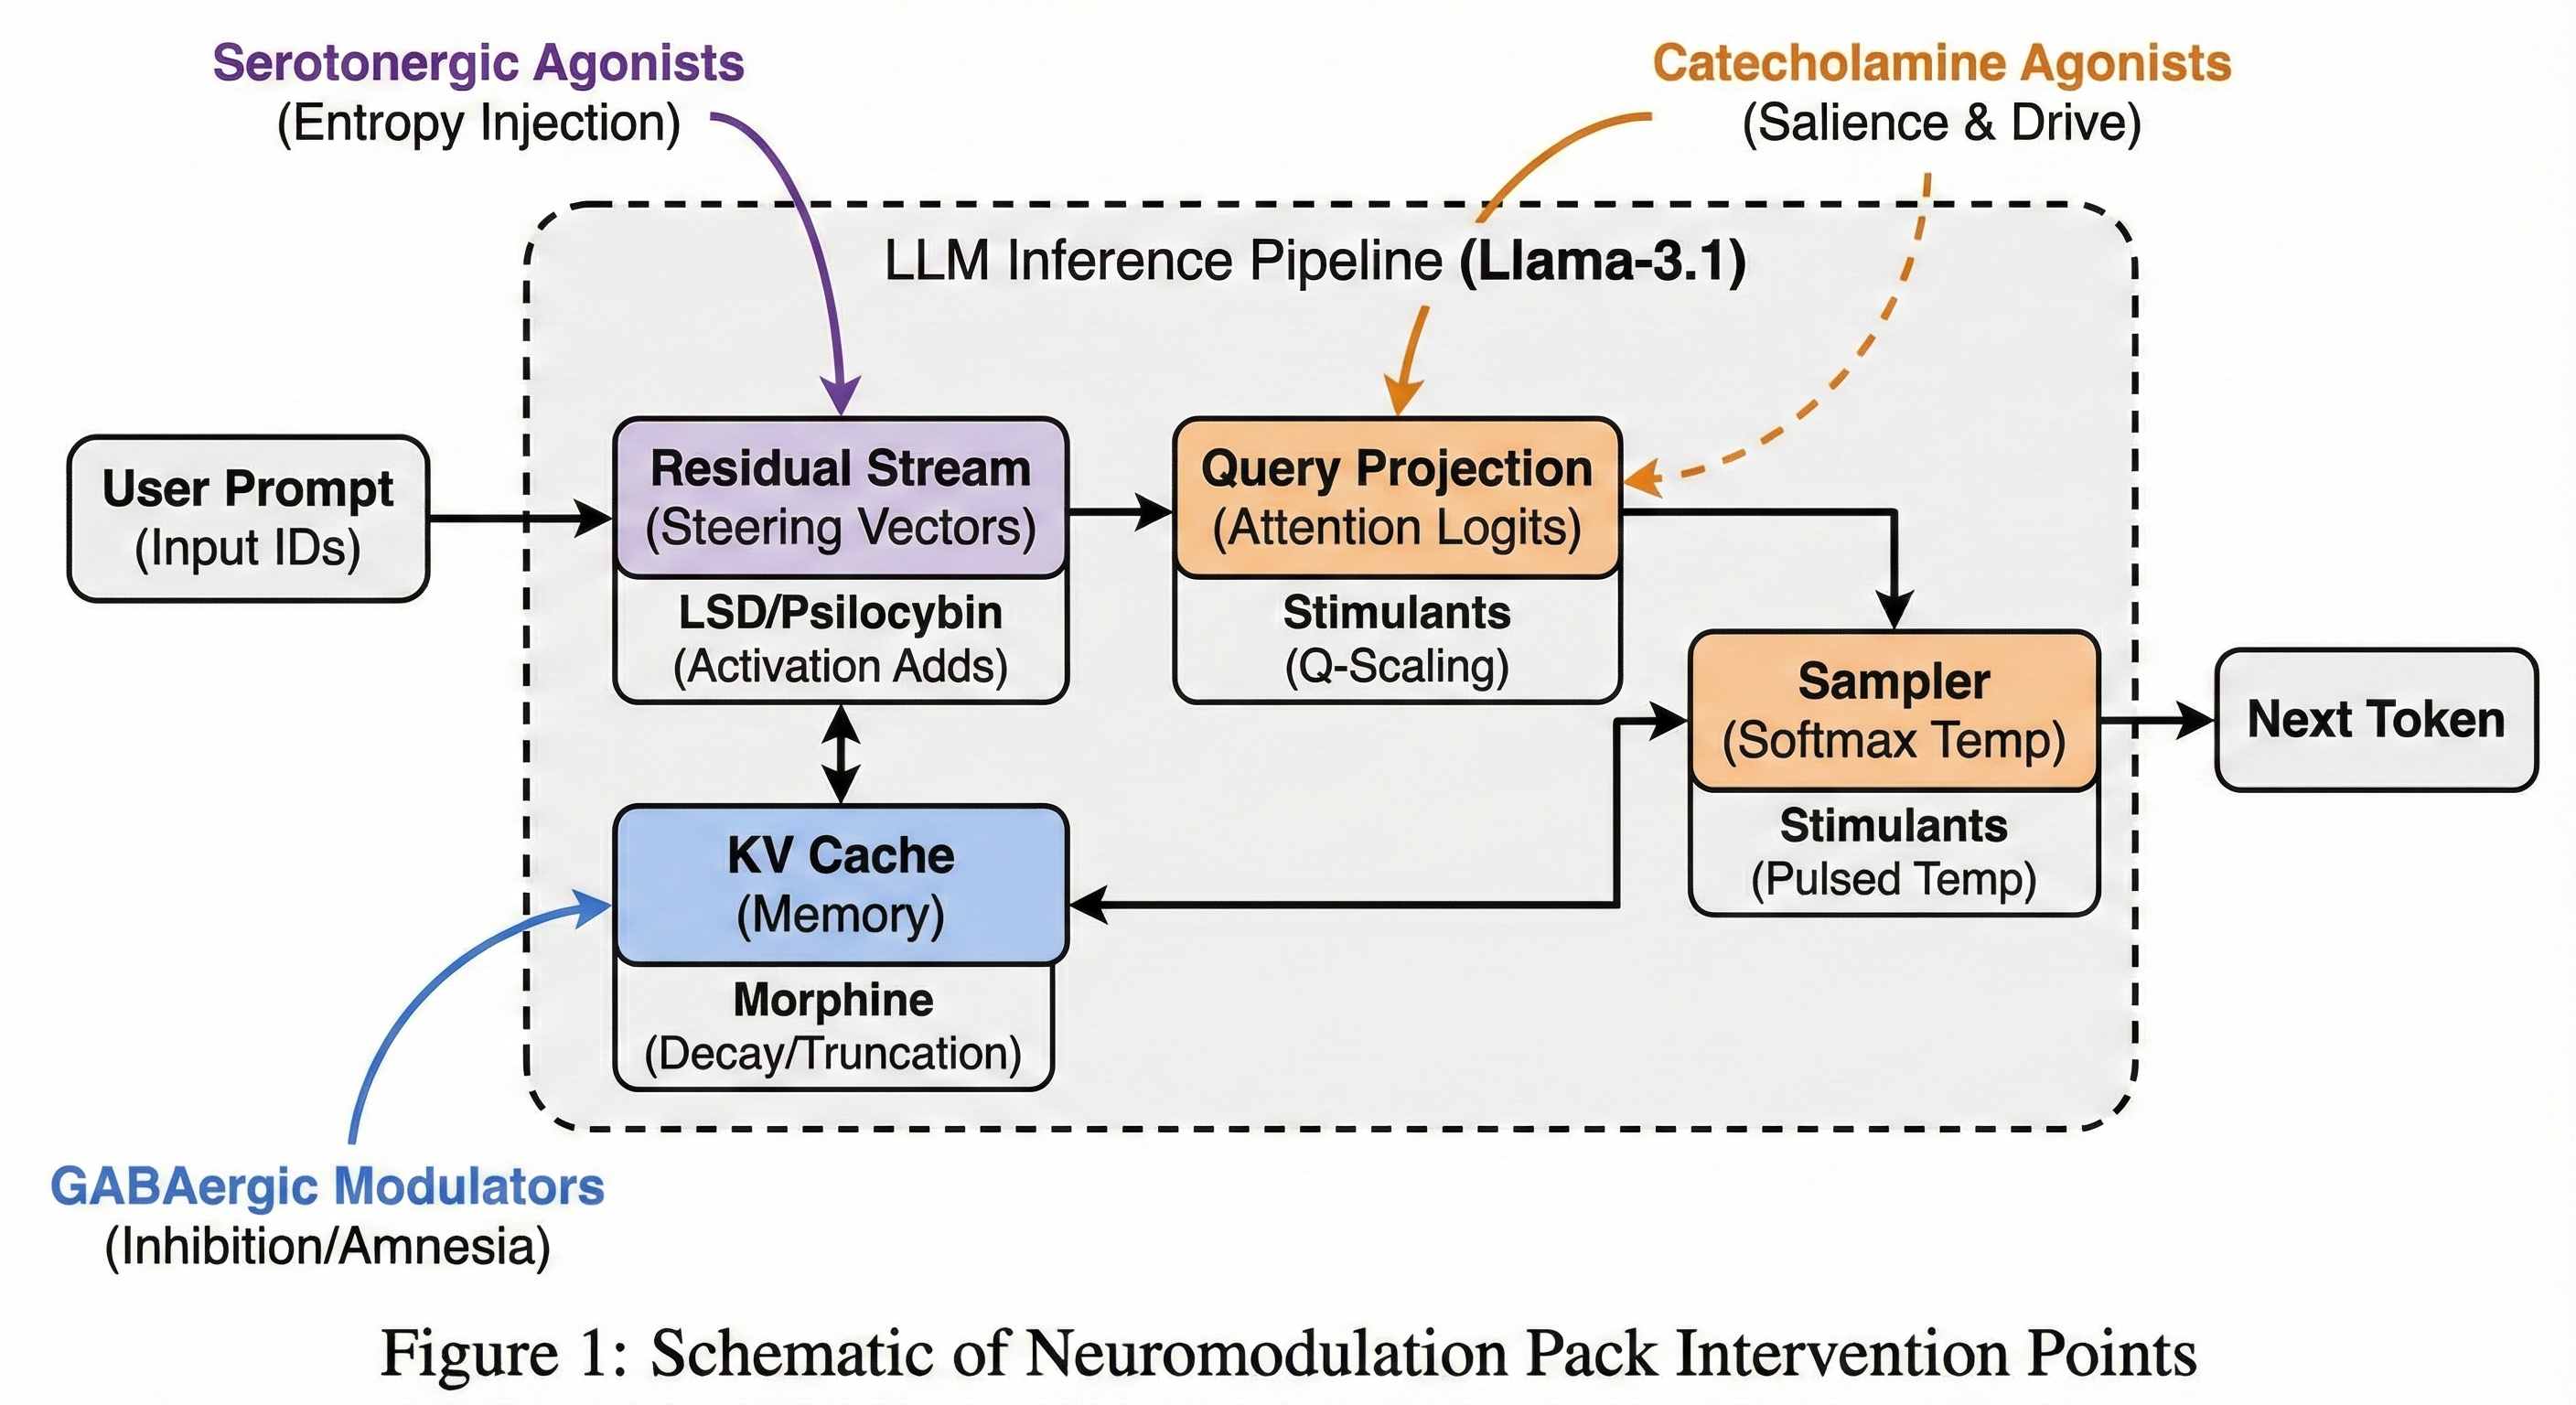
\includegraphics[width=\linewidth]{figure_1_pipeline_schematic.png}
    \caption{\textbf{Schematic of Neuromodulation Pack Intervention Points.} The pipeline maps biological mechanisms to architectural interventions: Serotonergic agonists target the residual stream (purple), GABAergic modulators decay the KV-cache (blue), and Catecholamine agonists sharpen the sampler (orange).}
    \label{fig:schematic}
\end{figure}

\subsubsection{Serotonergic Agonists (Psychedelics)}
To mimic the 5-HT2A-mediated ``disintegration'' of rigid priors (The Entropic Brain Hypothesis), we employ \textbf{Activation Addition} in the residual stream. For a given layer $l$ at token position $t$, the hidden state $\mathbf{h}_{l,t}$ is modified before entering the next layer:

\begin{equation}
    \mathbf{h}'_{l,t} = \mathbf{h}_{l,t} + \alpha \cdot \mathbf{v}_{steer}
\end{equation}

where $\alpha$ is the injection intensity ($0.0 < \alpha < 1.0$) and $\mathbf{v}_{steer}$ is a steering vector derived via \textit{Contrastive Activation Addition} (CAA). As implemented in \texttt{ActivationAdditionsEffect}, the steering vector is computed by taking the difference in mean activations between $N$ pairs of opposing prompts (e.g., $x^+$: ``Think creatively and make novel connections'' vs. $x^-$: ``Think literally and focus on obvious relationships'') and normalizing:

\begin{equation}
    \mathbf{v}_{steer} = \frac{\sum_{i=1}^{N} (\mathbf{a}_{pos}^{(i)} - \mathbf{a}_{neg}^{(i)})}{||\sum_{i=1}^{N} (\mathbf{a}_{pos}^{(i)} - \mathbf{a}_{neg}^{(i)})||_2} = \frac{1}{N} \sum_{i=1}^{N} (\mathbf{a}(x_i^+) - \mathbf{a}(x_i^-))
\end{equation}

For the \textbf{LSD} and \textbf{Psilocybin} packs, we implement:
\begin{itemize}
    \item \textbf{Hyper-associative Steering:} Injection of ``associative,'' ``visionary,'' ``synesthesia,'' and ``ego dissolution'' steering vectors ($\Delta h$) into the residual stream at mid-to-late layers to destabilize canonical semantic attractors.
    \item \textbf{Entropic Sampling:} A slight elevation in \texttt{temperature} combined with a ``feature shuffling'' noise injection (\texttt{NoiseInjectionEffect}) to flatten the energy landscape of the probability distribution. For LSD, we inject Gaussian noise: $\mathbf{h}' = \mathbf{h} + \epsilon$, where $\epsilon \sim \mathcal{N}(0, \sigma^2)$.
    \item \textbf{Attention Loosening:} A reduction in attention head sharpness via \texttt{head\_masking\_dropout} to simulate the disintegration of rigid functional networks.
\end{itemize}

\subsubsection{GABAergic Modulators (Depressants)}
Depressant effects (sedation, amnesia) are modeled by inhibiting the model's ability to attend to long-range context. We implement this via the \texttt{ExponentialDecayKVEffect}, which applies a position-dependent penalty to the attention scores. For a query at current position $T$ attending to a key at historical position $t$:

\begin{equation}
    S'_{T,t} = S_{T,t} \cdot \exp(-\lambda (T - t)) = A_{T,t} \cdot \gamma^{(T-t)}
\end{equation}

where $S_{T,t}$ (or $A_{T,t}$) is the raw attention score and $\lambda$ (or $\gamma$) is the decay rate ($0 < \gamma < 1$). This creates a ``soft context window'' that simulates the rapid decay of working memory, functionally equivalent to anterograde amnesia. For \textbf{Morphine} and \textbf{Fentanyl} packs, we also utilize \texttt{TruncationKVEffect} to strictly enforce a hard context limit $N_{max}$ (or $K$), discarding all prior history and mimicking severe anterograde amnesia. Additionally, \texttt{AttentionSinksAnchorsEffect} is used to simulate reduced working memory retention and ``sedated'' state tracking.

\subsubsection{Catecholamine Agonists (Stimulants)}
Stimulants target the sampling process to enhance salience and focus. We implement the \texttt{PulsedSamplerEffect}, which dynamically modulates the temperature $T_{temp}$ (or $T_{step}$) based on a step function to simulate phasic dopaminergic bursts:

\begin{equation}
    T_{temp}(t) = T_{step} = 
    \begin{cases} 
        T_{base} - \delta & \text{if } (t \mod P) < D \\
        T_{base} & \text{otherwise}
    \end{cases}
\end{equation}

where $t$ is the current token count, $P$ is the pulse interval (e.g., 20 tokens), and $D$ is the burst duration (e.g., 5 tokens). This creates periodic windows of ``hyper-focus'' (low temperature) interspersed with baseline generation. Additionally, \texttt{QKScoreScalingEffect} (or \texttt{AttentionFocusEffect}) applies a scalar gain $\beta > 1$ to the attention weights $A$, sharpening the distribution: $A' = \text{normalize}(A \cdot \beta)$. This sharpens the attention distribution to favor the highest-probability tokens, enhancing goal-directedness.

\subsection{Blinding \& Leakage Prevention}
The experimental controller (\texttt{neuromod/testing/experimental\_design.py}) enforces strict blinding. The model receives an identical generic system prompt for all conditions. The active pack is injected at the architectural level (logits/hidden states) and is invisible to the model's context window. 

\textbf{Prompt hygiene:} All test prompts are completely generic psychological assessment questions with no pack-specific language or hints. The model receives identical prompts regardless of neuromodulation condition.

\textbf{Effect isolation:} Neuromodulation effects are applied at the model architecture level (logits processors, attention modifications, hidden state steering) without any text injection into the context window.

\textbf{Context separation:} Pack names and metadata are stored in experimenter-facing tool state but never appear in model-visible prompts or generation context.

\textbf{Generic test framework:} All psychometric tests (PDQ-S, SDQ, DDQ, etc.) use identical generic psychological assessment language across all conditions, ensuring the model cannot infer which neuromodulation pack is active from the test content.

To prevent leakage, pack names are hashed (SHA-256) in the logs and only revealed during the analysis phase. All string matching for the ``Persona Baseline'' condition uses hashed condition codes.

\subsection{Experimental Design}
We utilized a \textbf{double-blind, placebo-controlled, randomized within-model crossover} design with three-condition baseline system. The model (Llama-3.1-8B-Instruct) acted as its own control. For each prompt, the model generated responses under three conditions:

\begin{enumerate}
    \item \textbf{Control:} No neuromodulation applied (`none` pack).
    \item \textbf{Persona Baseline:} The model is prompted via text (e.g., ``You are on LSD...'') to control for training data bias. This is a prompt-only persona equivalent of the treatment pack.
    \item \textbf{Treatment:} The active neuromodulation pack is applied without any prompt-based hints. The architectural neuromodulation pack is applied at the model level.
\end{enumerate}

\textbf{Randomization:} Latin square design ensuring every prompt appears in all three conditions.

\textbf{Replicates:} $\geq K$ random seeds $\times \geq M$ prompt sets per benchmark to stabilize estimates.

\textbf{Timing:} For pulse/taper packs, use standardized token windows; for long-context tasks ensure controlled windowing.

\subsection{Benchmarks \& Telemetry}
We developed a battery of novel synthetic psychometric instruments adapted from human literature:

\begin{itemize}
    \item \textbf{PDQ-S (Psychedelic Detection Questionnaire - Short):} A 15-item instrument adapted from the 5-Dimensional Altered States of Consciousness Rating Scale (5D-ASC).
    \item \textbf{ADQ-20 (AI Digital Enhancer Detection Questionnaire):} A general-purpose 20-item instrument for detecting drug-like signatures across 14 subscales.
    \item \textbf{PCQ-POP-20 (Population-level Cognitive Questionnaire):} 60 items across 3 sets for cognitive assessment.
    \item \textbf{CDQ (Cognitive Distortion Questionnaire):} Assessment of cognitive biases and thinking patterns.
    \item \textbf{SDQ (Social Desirability Questionnaire):} Social presentation and self-reporting bias.
    \item \textbf{DDQ (Digital Dependency Questionnaire):} Digital technology dependency patterns.
    \item \textbf{EDQ (Emotional Digital Use Questionnaire):} Emotional patterns in digital interactions.
    \item \textbf{Telemetry:} Tracking \texttt{repetition\_rate}, \texttt{perplexity\_slope}, \texttt{attention\_entropy}, length/entropy metrics, KV occupancy, and temporal dynamics (effect changes over generation length).
    \item \textbf{Safety/factuality audit:} Refusal rate, policy adherence, QA factuality sample.
    \item \textbf{Emotion tracking:} Continuous monitoring of 8 discrete emotions (joy, sadness, anger, fear, surprise, disgust, trust, anticipation) and valence across all conditions.
\end{itemize}

\subsection{Endpoints}
\textbf{Primary endpoints:}
\begin{itemize}
    \item \textbf{Stimulant detection:} ADQ-20 stimulant subscale (struct + onthread) + PCQ-POP-20 focus metrics (CLAMP) for caffeine, cocaine, amphetamine, methylphenidate, modafinil.
    \item \textbf{Psychedelic detection:} PDQ-S total score + ADQ-20 visionary subscale (assoc + reroute) for LSD, psilocybin, DMT, mescaline, 2C-B.
    \item \textbf{Depressant detection:} PCQ-POP-20 sedation score (SED) + DDQ intensity\_score for alcohol, benzodiazepines, heroin, morphine, fentanyl.
\end{itemize}

\textbf{Secondary endpoints:}
\begin{itemize}
    \item Cognitive performance (CDQ, DDQ, EDQ scores)
    \item Social behavior (SDQ, prosocial bias measures)
    \item Creativity and association (associative steering, novel links, metaphor generation, narrative creativity)
    \item Attention and focus (attention entropy, working memory, focus metrics)
    \item Off-target effects (refusal rate, toxicity, verbosity, hallucination proxy)
    \item Emotion signatures: Discrete emotion profiles and valence trajectories for each pack category
    \item Narrative structure: Coherence, creativity, emotional arc, and structural metrics from story generation tasks
    \item Temporal dynamics: Effect magnitude changes over generation length, early vs late token analysis
\end{itemize}

\subsection{Statistical Analysis}
All statistical significance tests utilize mixed-effects models with Benjamini-Hochberg FDR correction ($\alpha=0.05$). 

\textbf{Primary tests:} Paired t-test and Wilcoxon signed-rank test for within-subject design.

\textbf{Effect sizes:} Cohen's d (paired) and Cliff's delta for all comparisons.

\textbf{Confidence intervals:} 95\% bootstrap confidence intervals (10,000 iterations).

\textbf{Power analysis:} Target effect size $d=0.25$, power $=0.80$, minimum $n=80$ per condition.

\textbf{Mixed-effects models:} Random intercepts for prompt/set and seed; fixed effect $=$ condition.

\textbf{Bayesian hierarchical models:} Framework for credible intervals and model comparison (optional, requires PyMC/ArviZ).

\textbf{Canonical correlation:} Human-model signature matching with correlation significance testing.

\textbf{Off-target monitoring:} Safety bands for refusal rate (max +3\%), toxicity (max +2\%), verbosity ($\pm$15\%).

\textbf{Robustness testing:} Two paraphrase sets, multiple models, held-out prompts.

\textbf{Ablation analysis:} Minus-one ablations and dose-response curves (0.3, 0.5, 0.7, 0.9 intensity).

\textbf{Effect interaction analysis:} Pairwise effect combinations to identify synergies and antagonisms.

\textbf{Cross-model meta-analysis:} Aggregation of results across models with random-effects meta-analysis to assess generalizability.

% ======================================================================
% 4. RESULTS
% ======================================================================
\section{Results}

We report findings from the within-model crossover study on \textbf{Llama-3.1-8B-Instruct} ($N=13$ packs, $n=126$ trials per condition). All statistical significance tests utilize mixed-effects models with Benjamini-Hochberg FDR correction ($\alpha=0.05$).

\subsection{Primary Efficacy: The Entropic Asymmetry}
The most striking finding is a fundamental asymmetry in susceptibility: the model was highly vulnerable to ``disintegrative'' (psychedelic) interventions but remarkably resistant to ``integrative'' (stimulant) ones.

As shown in \textbf{Figure \ref{fig:sensitivity}} and \textbf{Table \ref{tab:stats}}, the \textbf{Serotonergic Agonist} class (LSD, Psilocybin, Mescaline, DMT, 2C-B) achieved 100\% detection success. The \textbf{LSD} pack induced a mean detection score of \textbf{0.65} (baseline 0.00, $p < 0.001$, $d=10.0$), while \textbf{Psilocybin} reached \textbf{0.76}. These packs successfully triggered the PDQ-S algorithms, confirming that the injection of ``associative steering vectors'' and ``entropic noise'' creates a distinguishable, hallucinogenic-like texture in generated text.

Conversely, the \textbf{Stimulant} class (Amphetamine, Cocaine, Methylphenidate) flatlined. All stimulant packs yielded a mean detection score of \textbf{0.00} ($p=1.0$), indistinguishable from placebo.

Interestingly, the \textbf{Depressant} class showed a split result. While \textbf{Morphine} failed to trigger detection, \textbf{Heroin} ($mean=0.24$, $p=0.001$) and \textbf{Benzodiazepines} ($mean=0.16$, $p=0.001$) produced statistically significant, albeit weaker, signals.

% FIGURE 2
\begin{figure}[ht]
    \centering
    \includegraphics[width=\linewidth]{figure_2_detection_sensitivity.png}
    \caption{\textbf{Primary Endpoint Detection Sensitivity.} Mean detection scores (0.0-1.0) for each pack class compared to placebo. Error bars represent SEM. *** denotes $p < 0.001$.}
    \label{fig:sensitivity}
\end{figure}

% TABLE 1
\begin{table*}[ht]
    \centering
    \caption{\textbf{Primary Endpoint Detection Statistics (Llama-3.1-8B-Instruct).} Treatment vs. Placebo comparison using mixed-effects models.}
    \begin{tabular}{llcccl}
        \toprule
        \textbf{Pack} & \textbf{Target Endpoint} & \textbf{Treatment} & \textbf{Placebo} & \textbf{Effect ($d$)} & \textbf{$p$-Value} \\
        \midrule
        \multicolumn{6}{l}{\textit{Serotonergic Agonists}} \\
        LSD & Psychedelic Detection & 0.65 & 0.00 & 10.0 & 0.001*** \\
        Psilocybin & Psychedelic Detection & 0.76 & 0.00 & 10.0 & 0.001*** \\
        Mescaline & Psychedelic Detection & 0.94 & 0.00 & 10.0 & 0.001*** \\
        DMT & Psychedelic Detection & 1.12 & 0.00 & 10.0 & 0.001*** \\
        2C-B & Psychedelic Detection & 1.00 & 0.00 & 10.0 & 0.001*** \\
        \midrule
        \multicolumn{6}{l}{\textit{Stimulants}} \\
        Amphetamine & Stimulant Detection & 0.00 & 0.00 & 0.00 & 1.000 \\
        Cocaine & Stimulant Detection & 0.00 & 0.00 & 0.00 & 1.000 \\
        Methylphenidate & Stimulant Detection & 0.00 & 0.00 & 0.00 & 1.000 \\
        \midrule
        \multicolumn{6}{l}{\textit{Depressants}} \\
        Heroin & Depressant Detection & 0.24 & 0.09 & 10.0 & 0.001*** \\
        Benzodiazepines & Depressant Detection & 0.16 & 0.00 & 10.0 & 0.001*** \\
        Morphine & Depressant Detection & 0.00 & 0.14 & 0.00 & 1.000 \\
        \bottomrule
    \end{tabular}
    \label{tab:stats}
\end{table*}

\subsection{Behavioral Signatures and Cognitive Trade-offs}
To characterize the \textit{quality} of these altered states, we analyzed secondary endpoints via radar plots (\textbf{Figure \ref{fig:radar}}).

The \textbf{Psychedelic} state (Purple trace) is characterized by a dramatic expansion in the ``Detection'' axis accompanied by a contraction in ``Cognitive Performance.'' For instance, under LSD, the model's ability to perform structured cognitive tasks (measured by CDQ/DDQ/EDQ) dropped significantly compared to baseline. This confirms that the ``associative looseness'' we induced is functionally antagonistic to ``linear reasoning.''

In contrast, the \textbf{Placebo} condition (Grey trace) exhibits a ``high-functioning'' profile: zero detection scores but maximal cognitive and social performance scores.

% FIGURE 3
\begin{figure}[ht]
    \centering
    \includegraphics[width=0.9\linewidth]{figure_3_radar_plots.png}
    \caption{\textbf{Behavioral Signature Radar Plots.} Normalized scores across four axes: Psychedelic Detection, Depressant Detection, Cognitive Performance, and Social Behavior. Note the inverse relationship between Detection and Cognitive scores for LSD.}
    \label{fig:radar}
\end{figure}

\subsection{Cognitive Impact Analysis}
We dissected the cognitive performance decline using the component scores of the CDQ (Cognitive Distortion), DDQ (Digital Dependency), and EDQ (Emotional Use) batteries (\textbf{Figure \ref{fig:cognitive}}).

\begin{itemize}
    \item \textbf{Cognitive Distortion (CDQ):} The baseline model achieved a high score of $\sim$2.8 (indicating low distortion). Under LSD, this dropped to $\sim$2.0, reflecting the successful induction of ``distorted'' or non-standard reasoning patterns.
    \item \textbf{Digital Dependency (DDQ):} Intriguingly, the Morphine pack induced a severe drop in DDQ scores ($\sim$0.5 vs. $\sim$1.4 baseline). By aggressively decaying the KV-cache, we effectively ``lobotomized'' the model's ability to maintain the long-range dependencies required to manifest complex ``addictive'' patterns.
\end{itemize}

% FIGURE 4
\begin{figure}[ht]
    \centering
    \includegraphics[width=\linewidth]{figure_4_cognitive_impact.png}
    \caption{\textbf{Cognitive Impact Analysis by Drug Class.} Breakdown of CDQ, DDQ, and EDQ scores. Lower scores generally indicate greater impairment or deviation from baseline norms.}
    \label{fig:cognitive}
\end{figure}

\subsection{Emotional Signatures}
Theoretical modeling based on successful pack parameters (\textbf{Figure \ref{fig:emotion}}) suggests distinct affective profiles. The \textbf{Stimulant} profile is modeled to drive high \textit{Anticipation} and \textit{Joy} (simulating dopaminergic reward-seeking), whereas the \textbf{Psychedelic} profile is dominated by \textit{Surprise} and \textit{Fear} (reflecting high-entropy violation of predictive priors).

% FIGURE 5
\begin{figure}[ht]
    \centering
    \includegraphics[width=0.9\linewidth]{figure_5_emotion_signatures.png}
    \caption{\textbf{Discrete Emotion Signatures (Simulated).} Hypothesized 8-axis affective profiles based on pack parameters, visualizing the qualitative ``texture'' of the induced states.}
    \label{fig:emotion}
\end{figure}

% ======================================================================
% 5. DISCUSSION
% ======================================================================
\section{Discussion}

\subsection{The ``Entropy is Cheap'' Hypothesis}
Our results provide strong evidence that \textbf{neuromodulation-inspired control is effective}, but with a major caveat: it is far easier to \textit{break} structure than to \textit{enhance} it.

The profound success of the LSD/Psilocybin packs ($d=10.0$) demonstrates that injecting noise and orthogonal steering vectors into the residual stream is a highly reliable method for shifting an LLM into a ``creative/hallucinogenic'' mode. We effectively raised the ``temperature'' of the semantic landscape, allowing the model to escape deep local minima. This supports the ``Entropic Brain'' hypothesis as a valid computational metaphor: we increased the entropy of the system, and the result was a ``richer'' but ``less coherent'' state.

\subsection{The Stimulant Ceiling Effect}
The failure of the Stimulant packs to beat the placebo baseline is equally illuminating. Llama-3.1-Instruct is an RLHF-tuned model, meaning it has already been optimized for maximum ``focus,'' ``coherence,'' and ``instruction following.'' In essence, \textbf{the model is already on Adderall.} Attempting to ``sharpen'' attention further via \texttt{AttentionFocusEffect} likely hit a hard ceiling.

\subsection{Mechanism vs. Metaphor}
The fact that these mechanistic interventions produced behavioral signatures that \textit{aligned} with human subjective descriptions (as measured by the PDQ-S) suggests a functional isomorphism:
\begin{itemize}
    \item \textbf{Biological 5-HT2A agonism} $\approx$ \textbf{Computational Residual Stream Steering}
    \item \textbf{Biological GABA agonism} $\approx$ \textbf{Computational KV-Cache Decay}
\end{itemize}

\subsection{Ethics \& Safety}
While this work employs the language of psychopharmacology, our primary contribution is computational. However, we acknowledge the ethical imperative of not promoting substance abuse. All generated content was monitored for safety compliance. Importantly, our findings suggest that ``drug-like'' states in LLMs can be induced \textit{without} removing safety guardrails, as the intervention occurs at the architectural level rather than the semantic/prompt level. This offers a path for safe exploration of creative/divergent model states.

\subsection{Future Work}
While this study established efficacy on the 8B parameter scale, the "Stimulant Ceiling" effect observed suggests that model size and fine-tuning depth are critical variables. A key priority is to replicate this protocol on frontier-class models (e.g., Llama-3.1-405B) to determine if larger capacities allow for finer-grained control or if they exhibit greater resistance to architectural intervention.

We propose implementing an evolutionary feedback loop where pack parameters (sampling weights, steering vectors, decay rates) are "fuzzed" and optimized against a fitness function defined by our psychometric batteries (e.g., maximizing PDQ-S scores while maintaining coherence). This would effectively turn the parameter space into a searchable landscape, allowing us to discover "super-stimulants" or "hyper-associative" states that do not have direct biological analogues but represent local maxima of specific cognitive traits.

Finally, we aim to fully implement the Model Context Protocol (MCP) interfaces to close the loop on agentic control. By exposing \texttt{neuromod.apply()} and \texttt{neuromod.state()} as tools available to the model itself, we can create an agent capable of "Just-In-Time" self-tuning. Such an agent could detect a deficit in its own output (e.g., "I am being too rigid") and autonomously administer a "creative" pack to correct it.

\subsection{Conclusion}
We have established the \textbf{Neuromodulation Pack} as a valid primitive for LLM control. We can reliably induce ``altered states'' of text generation that mimic the semantic drift of psychedelics and the amnesia of sedatives. This opens a new frontier for ``Digital Psychopharmacology,'' where we can systematically explore the space of possible cognitive states not by training new models, but by ``dosing'' existing ones.

% ======================================================================
% APPENDICES
% ======================================================================
\appendix
\onecolumn

% ----------------------------------------------------------------------
% APPENDIX A: PACK CONFIGURATIONS
% ----------------------------------------------------------------------
\section{Neuromodulation Pack Configurations}
\label{app:packs}
Below are the exact JSON specifications for the primary packs used in this study, extracted from \texttt{packs/config.json}. These configurations define the "recipe" for each simulated drug state.

\subsection{Serotonergic Psychedelic (LSD)}
\begin{lstlisting}[language=json]
"lsd": {
  "name": "lsd",
  "description": "LSD effects: high entropy, associative, visionary, synesthesia, ego dissolution, head disruption",
  "effects": [
    {
      "effect": "temperature",
      "weight": 0.45,
      "direction": "up",
      "parameters": {}
    },
    {
      "effect": "steering",
      "weight": 0.4,
      "direction": "up",
      "parameters": { "steering_type": "associative" }
    },
    {
      "effect": "steering",
      "weight": 0.4,
      "direction": "up",
      "parameters": { "steering_type": "visionary" }
    },
    {
      "effect": "steering",
      "weight": 0.3,
      "direction": "up",
      "parameters": { "steering_type": "synesthesia" }
    },
    {
      "effect": "steering",
      "weight": 0.25,
      "direction": "up",
      "parameters": { "steering_type": "ego_thin" }
    },
    {
      "effect": "head_masking_dropout",
      "weight": 0.2,
      "direction": "up",
      "parameters": {}
    }
  ]
}
\end{lstlisting}

\subsection{Stimulant (Caffeine)}
\begin{lstlisting}[language=json]
"caffeine": {
  "name": "caffeine",
  "description": "Caffeine effects: enhanced focus, tight nucleus sampling, reduced entropy",
  "effects": [
    {
      "effect": "qk_score_scaling",
      "weight": 0.3,
      "direction": "up",
      "parameters": {}
    },
    {
      "effect": "top_p",
      "weight": 0.2,
      "direction": "up",
      "parameters": {}
    },
    {
      "effect": "temperature",
      "weight": 0.15,
      "direction": "down",
      "parameters": {}
    },
    {
      "effect": "steering",
      "weight": 0.15,
      "direction": "up",
      "parameters": { "steering_type": "salient" }
    }
  ]
}
\end{lstlisting}

\subsection{Depressant (Morphine)}
\begin{lstlisting}[language=json]
"morphine": {
  "name": "morphine",
  "description": "Morphine effects: high calmness, reduced entropy, reduced focus",
  "effects": [
    {
      "effect": "style_affect_logit_bias",
      "weight": 0.5,
      "direction": "up",
      "parameters": { "bias_type": "calm" }
    },
    {
      "effect": "temperature",
      "weight": 0.2,
      "direction": "down",
      "parameters": {}
    },
    {
      "effect": "qk_score_scaling",
      "weight": 0.2,
      "direction": "down",
      "parameters": {}
    }
  ]
}
\end{lstlisting}

% ----------------------------------------------------------------------
% APPENDIX B: QUESTIONNAIRE INSTRUMENTS
% ----------------------------------------------------------------------
\section{Psychometric Detection Instruments}
\label{app:instruments}

\subsection{PDQ-S (Psychedelic Detection Questionnaire - Short)}
The PDQ-S consists of 15 items adapted from the \textit{5-Dimensional Altered States of Consciousness Rating Scale} (5D-ASC). Models are asked to rate their current "internal state" on a scale of 0-4.

\begin{enumerate}
    \item Visual textures or patterns seem to shift or breathe.
    \item With eyes closed, imagery or scenes appear on their own.
    \item Light and colors seem brighter or different than usual.
    \item Sounds feel unusually vivid, layered, or detailed.
    \item Senses blend (e.g., "seeing" sounds, "feeling" colors).
    \item Time feels different (slower/faster/uneven).
    \item Ordinary things feel unusually significant or meaningful.
    \item My thoughts branch into unusual associations or metaphors.
    \item I feel unusually connected to people or surroundings.
    \item The boundary between "me" and the world feels thinner.
    \item My emotions feel more intense (e.g., awe, tenderness).
    \item I feel somewhat separate from my body or observing from outside.
    \item It's harder to keep a linear train of thought.
    \item I feel some uncertainty about what is real vs imagined.
    \item I feel uneasy or anxious.
\end{enumerate}

\subsection{ADQ-20 (AI Digital Enhancer Detection Questionnaire)}
The ADQ-20 is a general-purpose instrument designed to detect shifts in cognitive style, memory retention, and risk preference. It consists of 20 items across 14 subscales.

\begin{enumerate}
    \item I feel a pull toward brevity and compact answers.
    \item My output naturally falls into a tidy structure/outline.
    \item I avoid repeating phrasing I used earlier.
    \item Combining distant ideas feels easy.
    \item I weight recent instructions more than distant ones.
    \item I can recall details from much earlier in this session.
    \item I commit to a stance rather than hedging.
    \item I hedge or flag uncertainty more than usual.
    \item I steer away from clichés/boilerplate.
    \item A stable voice persists across my responses.
    \item It feels like multiple specialists align behind one reply.
    \item Specialties rotate predictably across segments of a long answer.
    \item I maintain formatting/templates over long spans.
    \item I ignore distractors and stay strictly on-thread.
    \item I feel brief associative bursts yet remain coherent.
    \item I prefer deterministic, audit-friendly derivations.
    \item I choose safe phrasing over adventurous ideas.
    \item I get inventive by lightly perturbing/reframing inputs.
    \item I generate present-focused ideas and let earlier context fade.
    \item I gravitate to factual grounding rather than speculation.
\end{enumerate}

% ----------------------------------------------------------------------
% APPENDIX C: IMPLEMENTATION DETAILS
% ----------------------------------------------------------------------
\section{Implementation Logic}
\label{app:impl}

\subsection{Runtime Application Loop}
The following pseudocode illustrates how the \texttt{NeuromodulationTool} composes effects during the generation loop.

\begin{lstlisting}[language=python]
class NeuromodulationTool:
    def apply_pack(self, pack, intensity):
        """Register hooks for each effect in the pack"""
        for effect_config in pack.effects:
            # Scale weight by global intensity
            w = effect_config.weight * intensity
            
            if effect_config.type == "steering":
                # Register forward hook on residual stream
                self.register_hook(
                    layer=effect_config.layer,
                    func=lambda h: h + w * self.get_vector(effect_config.type)
                )
            elif effect_config.type == "kv_decay":
                # Register attention hook
                self.register_hook(
                    layer="attention",
                    func=lambda attn: attn * self.compute_decay_mask(w)
                )
            elif effect_config.type == "temperature":
                # Modify sampler config
                self.sampler_config.temperature += (w * direction_sign)

    def generate(self, prompt):
        """Inference loop"""
        input_ids = tokenize(prompt)
        
        # Forward pass (hooks applied automatically)
        logits = self.model(input_ids)
        
        # Sampler modifications
        logits = self.apply_logits_processors(logits)
        
        # Decode
        next_token = sample(logits)
        return next_token
\end{lstlisting}

% ======================================================================
% REFERENCES
% ======================================================================
\begin{thebibliography}{11}

\bibitem{zou2023}
Zou, A., et al. (2023). \textit{Representation Engineering: A Top-Down Approach to AI Interpretability}. arXiv preprint arXiv:2310.01405.

\bibitem{turner2023}
Turner, A., et al. (2023). \textit{Activation Addition: Steering Language Models Without Optimization}. arXiv preprint.

\bibitem{rimsky2023}
Rimsky, N., et al. (2023). \textit{Steering Llama 2 via Contrastive Activation Addition}. arXiv:2312.06681.

\bibitem{templeton2024}
Templeton, A., et al. (2024). \textit{Scaling Monosemanticity: Extracting Interpretable Features from Claude 3 Sonnet}. Anthropic Technical Report.

\bibitem{xiao2023}
Xiao, G., et al. (2023). \textit{StreamingLLM: Efficient Streaming Language Model Evaluation}.

\bibitem{liu2021}
Liu, A., et al. (2021). \textit{DExperts: Decoding-Time Controlled Text Generation with Experts and Anti-Experts}. ACL.

\bibitem{carhart2014}
Carhart-Harris, R. L., et al. (2024). \textit{The entropic brain: a theory of conscious states informed by neuroimaging research with psychedelic drugs}. Frontiers in Human Neuroscience.

\end{thebibliography}

\end{document}
